% Options for packages loaded elsewhere
\PassOptionsToPackage{unicode}{hyperref}
\PassOptionsToPackage{hyphens}{url}
\PassOptionsToPackage{dvipsnames,svgnames,x11names}{xcolor}
\documentclass[
  10pt,
  fontset=fandol]{ctexart}
\usepackage{xcolor}
\usepackage[margin=16mm]{geometry}
\usepackage{amsmath,amssymb}
\setcounter{secnumdepth}{-\maxdimen} % remove section numbering
\usepackage{iftex}
\ifPDFTeX
  \usepackage[T1]{fontenc}
  \usepackage[utf8]{inputenc}
  \usepackage{textcomp} % provide euro and other symbols
\else % if luatex or xetex
  \usepackage{unicode-math} % this also loads fontspec
  \defaultfontfeatures{Scale=MatchLowercase}
  \defaultfontfeatures[\rmfamily]{Ligatures=TeX,Scale=1}
\fi
\usepackage{lmodern}
\ifPDFTeX\else
  % xetex/luatex font selection
\fi
% Use upquote if available, for straight quotes in verbatim environments
\IfFileExists{upquote.sty}{\usepackage{upquote}}{}
\IfFileExists{microtype.sty}{% use microtype if available
  \usepackage[]{microtype}
  \UseMicrotypeSet[protrusion]{basicmath} % disable protrusion for tt fonts
}{}
\makeatletter
\@ifundefined{KOMAClassName}{% if non-KOMA class
  \IfFileExists{parskip.sty}{%
    \usepackage{parskip}
  }{% else
    \setlength{\parindent}{0pt}
    \setlength{\parskip}{6pt plus 2pt minus 1pt}}
}{% if KOMA class
  \KOMAoptions{parskip=half}}
\makeatother
\usepackage{graphicx}
\makeatletter
\newsavebox\pandoc@box
\newcommand*\pandocbounded[1]{% scales image to fit in text height/width
  \sbox\pandoc@box{#1}%
  \Gscale@div\@tempa{\textheight}{\dimexpr\ht\pandoc@box+\dp\pandoc@box\relax}%
  \Gscale@div\@tempb{\linewidth}{\wd\pandoc@box}%
  \ifdim\@tempb\p@<\@tempa\p@\let\@tempa\@tempb\fi% select the smaller of both
  \ifdim\@tempa\p@<\p@\scalebox{\@tempa}{\usebox\pandoc@box}%
  \else\usebox{\pandoc@box}%
  \fi%
}
% Set default figure placement to htbp
\def\fps@figure{htbp}
\makeatother
\setlength{\emergencystretch}{3em} % prevent overfull lines
\providecommand{\tightlist}{%
  \setlength{\itemsep}{0pt}\setlength{\parskip}{0pt}}
\usepackage{amsmath,amssymb,mathtools,needspace}
\xeCJKDeclareCharClass{CJK}{"2032,"0400->"04FF,"2160->"216B,"2460->"2473,"25A0,"25C7,"25CB,"25CF}
\IfFontExistsTF{Arial Unicode MS}{\xeCJKsetup{AutoFallBack=true}\setCJKfallbackfamilyfont{\CJKrmdefault}{Arial Unicode MS}}{}
\setcounter{secnumdepth}{0}
\setlength{\emergencystretch}{2em}
\allowdisplaybreaks
\usepackage{bookmark}
\IfFileExists{xurl.sty}{\usepackage{xurl}}{} % add URL line breaks if available
\urlstyle{same}
\hypersetup{
  pdftitle={抛物线法},
  colorlinks=true,
  linkcolor={Maroon},
  filecolor={Maroon},
  citecolor={Blue},
  urlcolor={Blue},
  pdfcreator={LaTeX via pandoc}}

\title{抛物线法}
\author{}
\date{}

\begin{document}
\maketitle

\subsubsection{6.4.2 抛物线法}\label{ux629bux7269ux7ebfux6cd5}

设已知方程 \(f(x)=0\) 的三个近似根 \(x_k,x_{k-1},x_{k-2}\)，以这三点为节点构造二次插值多项式 \(P_2(x)\)，并适当选取 \(P_2(x)\) 的一个零点 \(x_{k+1}\) 作为新的近似根，这样确定的迭

\begin{quote}
校注（agent 补充）：定理 6.4 的原文条件与 \(p=(1+\sqrt5)/2\) 结论均已保留。若将此处``按阶''理解为定义 6.2 中极限常数非零的精确收敛阶，还需 \(f''(x^*)\ne0\) 等非退化条件，并排除有限步已得根的情形。例如一次函数满足原定理的光滑性与导数非零条件，但弦截法可一步得根，不能一概赋予上述精确阶。
\end{quote}

\href{../../source-images/pdf-170.jpeg}{原页}

代过程称为抛物线法。在几何图形上，这种方法的基本思想是用抛物线 \(y=P_2(x)\) 与 \(x\) 轴的交点 \(x_{k+1}\) 作为所求根 \(x^*\) 的近似位置（见图 6.6）。

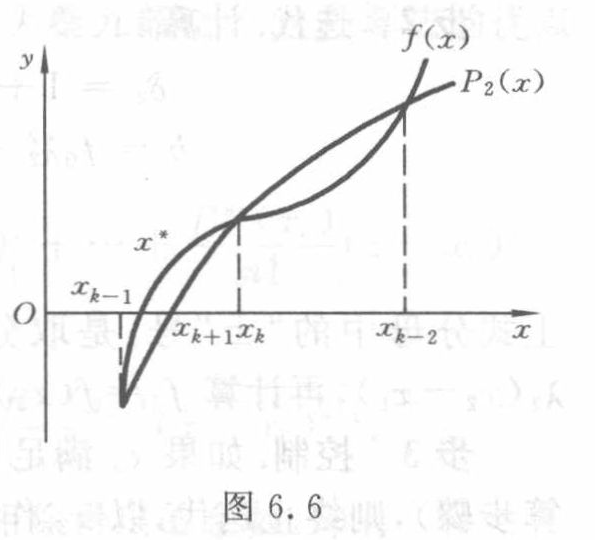
\includegraphics[width=0.85\linewidth,height=\textheight,keepaspectratio,alt={图 6.6 原扫描裁切}]{../assets/ch06/fig-6.6.png}

图 6.6

图意（agent 整理）：原图以抛物线 \(P_2(x)\) 近似曲线 \(f(x)\)，用抛物线与 \(x\) 轴的交点作为新近似根。全部标签为 \(x,\allowbreak y,\allowbreak O,\allowbreak x^*,\allowbreak x_{k-1},\allowbreak x_{k+1},\allowbreak x_k,\allowbreak x_{k-2},\allowbreak f(x),\allowbreak P_2(x)\)。

现在推导抛物线法的计算公式。插值多项式

\[
\begin{aligned}
P_2(x)={}&f(x_k)+f[x_k,x_{k-1}](x-x_k)\\
&+f[x_k,x_{k-1},x_{k-2}](x-x_k)(x-x_{k-1})
\end{aligned}
\]

有两个零点

\[
x_{k+1}=x_k-\frac{2f(x_k)}{\omega\pm\sqrt{\omega^2-4f(x_k)f[x_k,x_{k-1},x_{k-2}]}},
\tag{6.4.3}
\]

其中

\[
\omega=f[x_k,x_{k-1}]+f[x_k,x_{k-1},x_{k-2}](x_k-x_{k-1}).
\]

为了从式（6.4.3）定出一个值 \(x_{k+1}\)，需要讨论根式前正负号的取舍问题。

在 \(x_k,x_{k-1},x_{k-2}\) 三个近似根中，自然假定以 \(x_k\) 更接近所求的根 \(x^*\)，这时，为了保证精度，可以选式（6.4.3）中较接近 \(x_k\) 的一个值作为新的近似根 \(x_{k+1}\)，为此，只要令根式前的符号与 \(\omega\) 的符号相同。

\textbf{例 6.10} 用抛物线法求解方程 \(f(x)=x\mathrm{e}^x-1=0\)。

\textbf{解} 设用表 6.9 中的前三个值 \(x_0=0.5,x_1=0.6,x_2=0.565\,32\) 作为开始值，计算得

\[
\begin{aligned}
f(x_0)&=-0.175\,639,& f(x_1)&=-0.093\,271,\\
f(x_2)&=-0.005\,031,& f[x_1,x_0]&=2.689\,10,\\
f[x_2,x_1]&=2.833\,73,& f[x_2,x_1,x_0]&=2.214\,18,
\end{aligned}
\]

故

\[
\omega=f[x_2,x_1]+f[x_2,x_1,x_0](x_2-x_1)=2.756\,94.
\]

代入式（6.4.8）求得

\[
x_3=x_2-\frac{2f(x_2)}{\omega+\sqrt{\omega^2-4f(x_2)f[x_2,x_1,x_0]}}=0.567\,14.
\]

以上计算表明，抛物线法比弦截法收敛得更快。

事实上，在一定条件下可以证明，对于抛物线法，迭代误差有下列渐近关系式：

\[
\frac{|e_{k+1}|}{|e_k|^{1.840}}\to\left|\frac{f'''(x^*)}{6f'(x^*)}\right|^{0.42},
\]

可见抛物线法也是超线性收敛的，其收敛的阶 \(p=1.840\)，收敛速度比弦截法更接近于 Newton 法。

下面列出抛物线法的计算步骤。

\textbf{步 1} 准备。选定初始近似值 \(x_0,x_1,x_2\)，并计算 \(f(x)\) 相应的值 \(f_0,f_1,f_2\)，以及

\[
\lambda_2=\frac{x_2-x_1}{x_1-x_0}.
\]

\begin{quote}
校注（agent 补充）：原页例 6.10 印为 \(f(x_1)=-0.093\,271\)，此处保留原文。由同页 \(x_1=0.6\) 和 \(f(x)=x\mathrm{e}^x-1\)，计算得 \(f(0.6)=0.093\,271\,280\ldots>0\)；同时 \([f(0.6)-f(0.5)]/0.1=2.689\,106\ldots\) 与原页列出的差商一致，因此原页该负号疑为误印。原页的``代入式（6.4.8）''也予保留；该段实际使用的零点公式编号是同页（6.4.3）。
\end{quote}

\href{../../source-images/pdf-171.jpeg}{原页}

\textbf{步 2} 迭代。计算

\[
\begin{aligned}
\delta_2&=1+\lambda_2,\quad a=f_0\lambda_2^2-f_1\lambda_2\delta_2+f_2\lambda_2,\\
b&=f_0\lambda_2^2-f_1\delta_2^2+f_2(\lambda_2+\delta_2),\quad c=f_2\delta_2,\\
\lambda_3&=\frac{-2c}{b\pm\sqrt{b^2-4ac}}.
\end{aligned}
\]

上式分母中的``\(\pm\)''号，是取分母的模较大的一个。于是得新的近似值 \(x_3=x_2+\lambda_3(x_2-x_1)\)，再计算 \(f_3=f(x_3)\)。

\textbf{步 3} 控制。如果 \(x_3\) 满足 \(|\delta|\leqslant\varepsilon_1\) 或 \(|f_3|<\varepsilon_2\)（\(\varepsilon_1,\varepsilon_2\) 和 \(\delta\) 的意义同弦截法的计算步骤），则终止迭代，以 \(x_3\) 作为所求的根；否则执行步 4。

\textbf{步 4} 修改。如果迭代次数达到预先指定的次数 \(N\)，则认为过程不收敛，输出计算失效标志；否则以 \((x_1,\allowbreak x_2,\allowbreak x_3,\allowbreak f_1,\allowbreak f_2,\allowbreak f_3,\allowbreak \lambda_3)\) 分别代替 \((x_0,\allowbreak x_1,\allowbreak x_2,\allowbreak f_0,\allowbreak f_1,\allowbreak f_2,\allowbreak \lambda_2)\) 转步 2 继续迭代。

\subsection{本节覆盖原页的校注记录}\label{ux672cux8282ux8986ux76d6ux539fux9875ux7684ux6821ux6ce8ux8bb0ux5f55}

下列记录按原页关联，含同页相邻小节的校注；计算时同时读取上文校注和完整原页。

\begin{itemize}
\tightlist
\item
  \texttt{ch06-E003}：原书 PDF 页 170
\item
  \texttt{ch06-E004}：原书 PDF 页 170
\item
  \texttt{ch06-E010}：原书 PDF 页 169
\end{itemize}

\end{document}
